\documentclass[11pt]{article}
\usepackage{amsmath,amssymb,amsfonts,epsfig,algorithm,algorithmic,url}

\textheight 8.8truein
\parskip 0.1in
\topmargin -0.5truein
\textwidth 6.5truein
\oddsidemargin -0.05in
\evensidemargin -0.05in
% \renewcommand{\baselinestretch}{1.2}   %line space adjusted here
\setcounter{footnote}{0}
\sloppy

\renewcommand{\theequation}{\thesection.\arabic{equation}}
\newcommand{\newsection}{\setcounter{equation}{0}\section}

% redefining commonly used symbols
\DeclareMathOperator{\trace}{Tr}

\newtheorem{theorem}{Theorem}
\newtheorem{proposition}[theorem]{Proposition}
\newtheorem{lemma}[theorem]{Lemma}
\newtheorem{corollary}[theorem]{Corollary}
\newtheorem{definition}[theorem]{Definition}
\newtheorem{example}[theorem]{Example}

\begin{document}
\title{\bf EE394V Data Analytics in Power Systems\\
	Project Title
}
\date{\today}
\author{Your Name}
%\normalsize{}
\maketitle

\begin{abstract}
	This is a \emph{recommended} template for both the 2-page project proposal (references can go over 2 pages) and the final project report. For the proposal, the abstract and some of the sections may be shortened or even skipped (e.g., Conclusions or Numerical Experiments Sections). In the abstract here, please give a high-level description of the problem, its application area, the challenges, preliminary data or results available for this problem, and what you are planning to do in the final project. Use less than 160 words in the final report.
\end{abstract}

\section{Introduction}\label{sec:intro}
A more detailed and technical version of the abstract. \textbf{Review of existing approaches} could be also included here. Literature review is a salient part of conducting research, so please look for online resources on how to prepare literature review if you are not certain. In the proposal phase, highlight the aspects that you look for investigating and potential benefits that may be expected. For the final report, clearly identify one to three contributions that you are targeting. 

\section{Problem Formulation}\label{sec:problem}
The proposal does not need detailed description of problem formulation that it should be a key section in the final project. 

Introduce the input data and parameters, problem variables (output), possible auxiliary variables. Introduce the problem statement with an objective. Comment on the availability of data (the data sources) or how you plan to generate synthetic data using simulation tools; review of existing approaches; or proposed work (machine learning/statistical estimation/performance analysis, etc). You can cite references by \cite{WWS,YGC02} for example.

\begin{figure}[htb]\label{fig:ed}
	\centering
	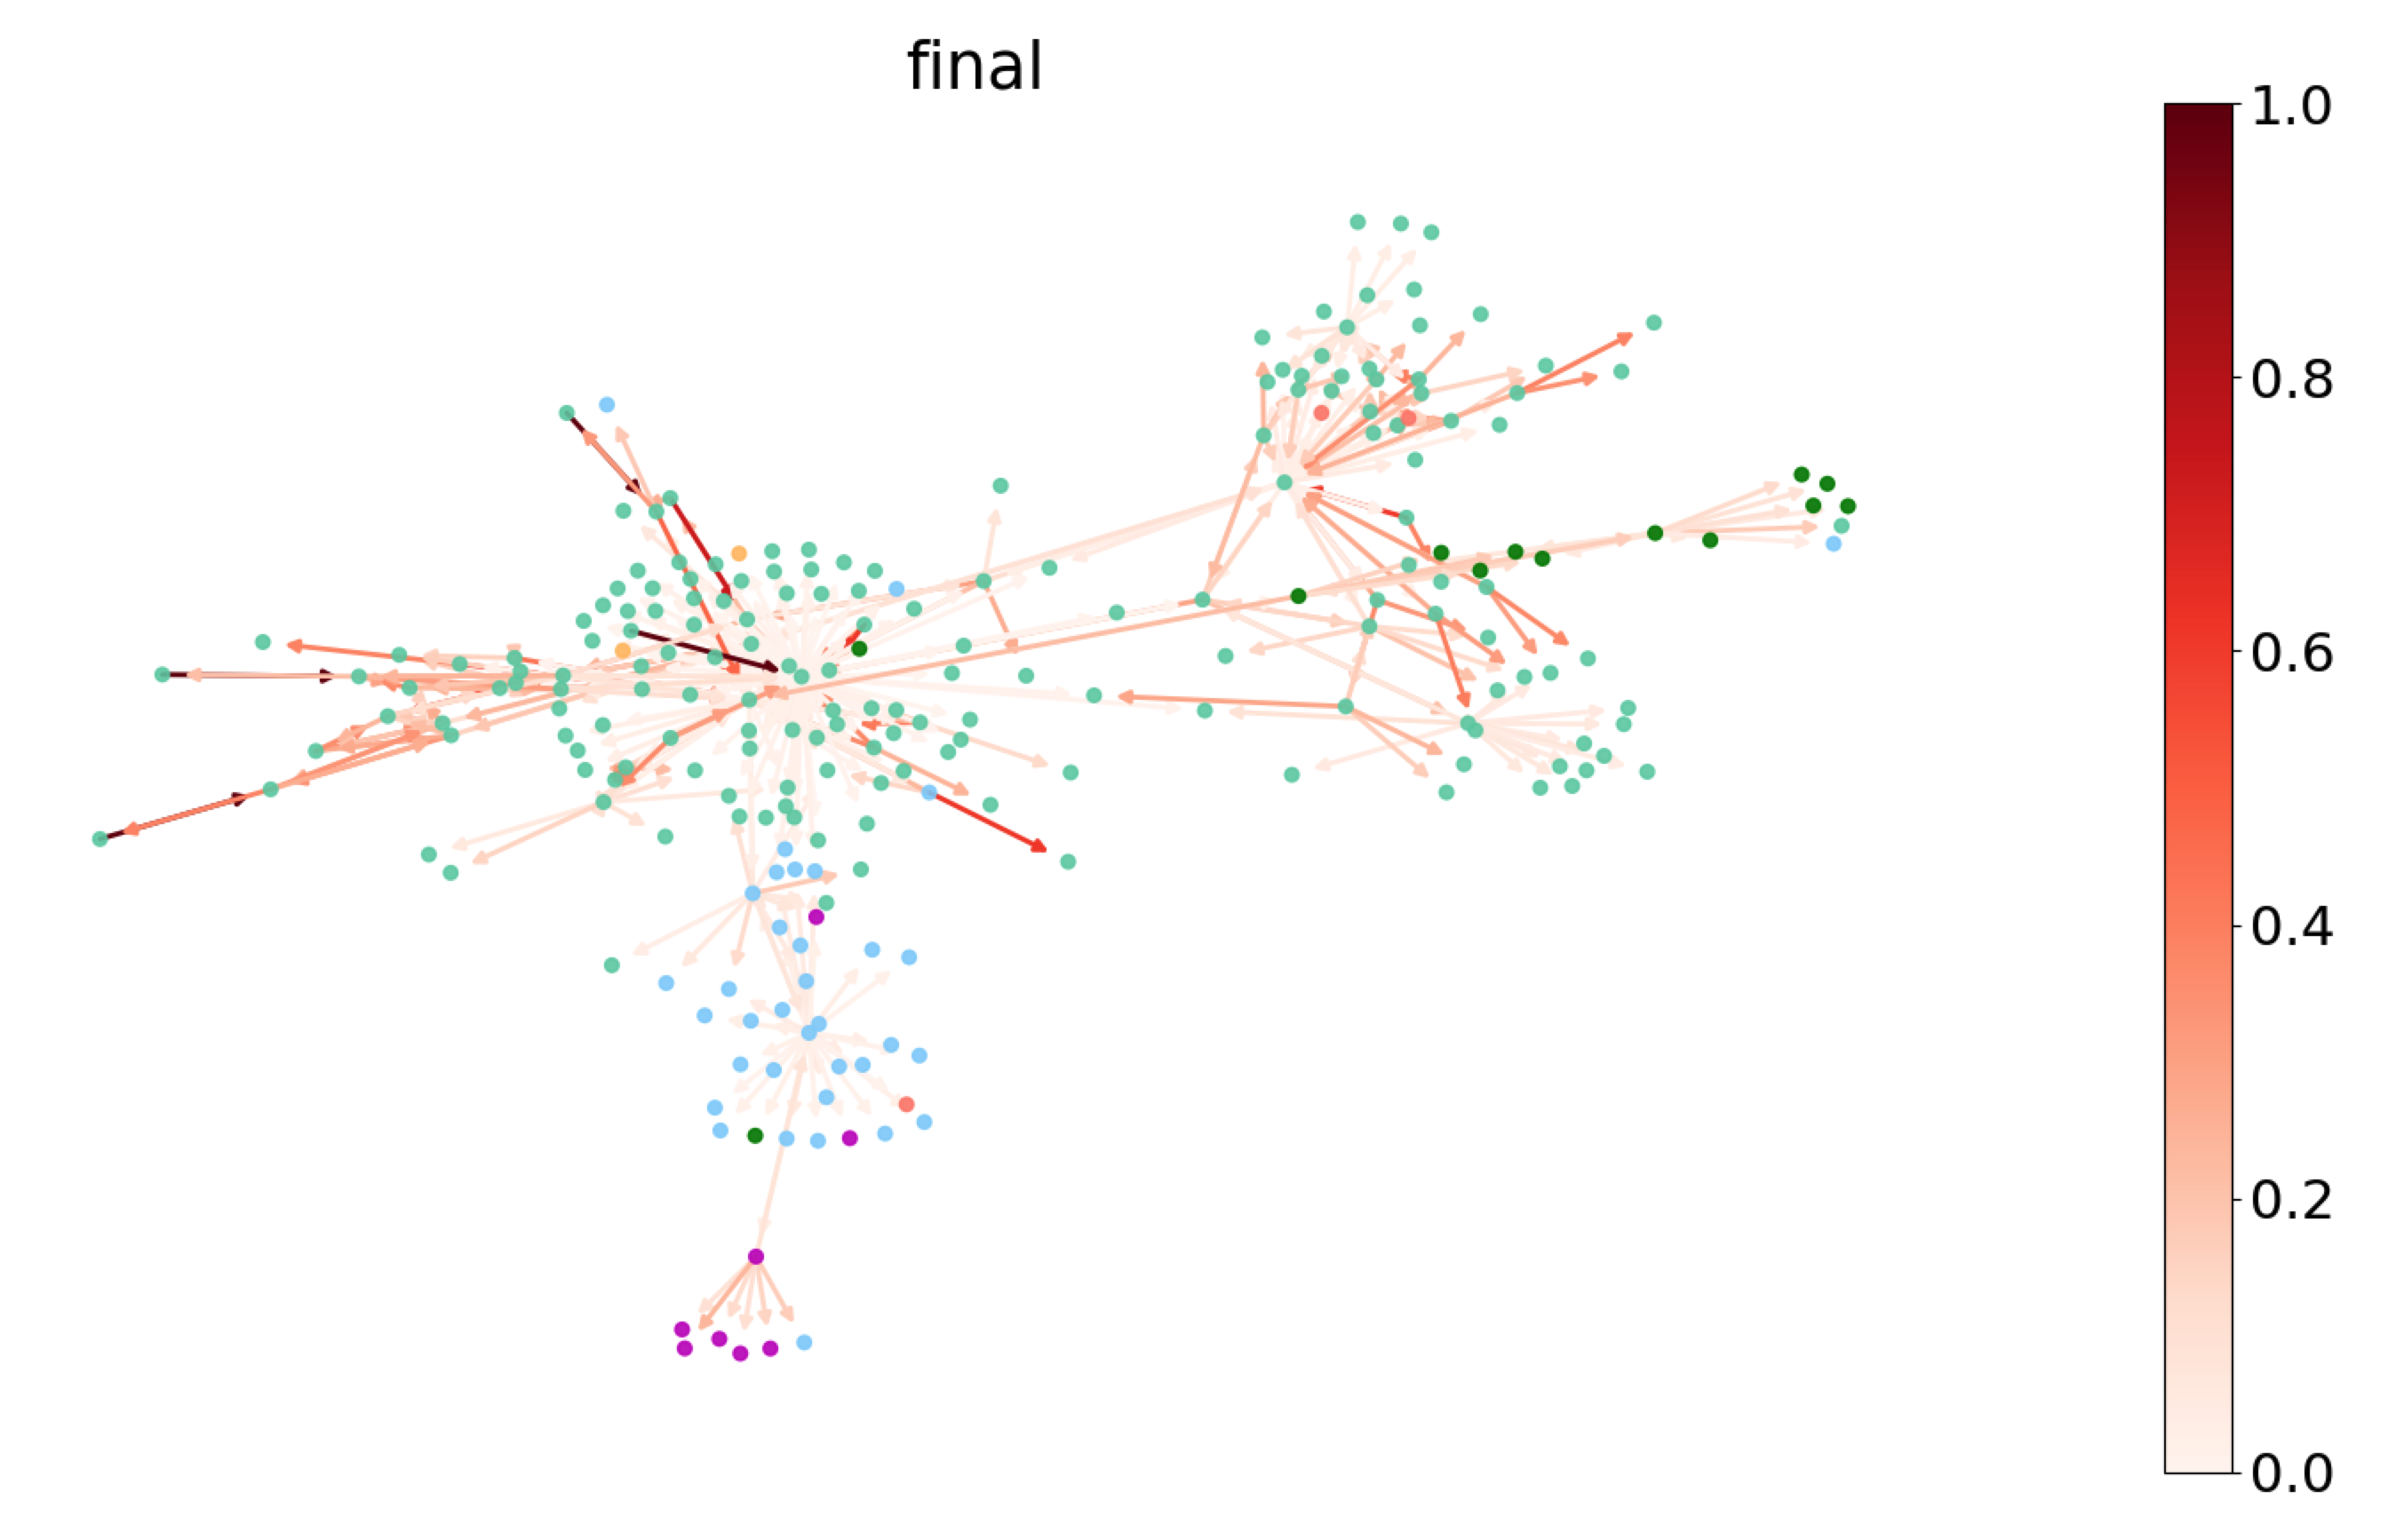
\includegraphics[scale=0.1]{etc/proposal/figures/eg of visualize gat attention weights.png}
	\caption{Sample figure.}
\end{figure}

\textbf{Equation examples}: In the dimensionality reduction problem, there are $N$ input data vectors $\{\mathbf x_n\}$, with each $\mathbf x_n\in \mathbb R^d$; see Figure~\ref{fig:ed} for the illustration of $d=2$. The goal is to find a linear projection such that each $\mathbf x_n$ is mapped to an $m$-dimensional subspace with $m\ll d$. Hence, the problem can be formulated as one to search for the orthonormal projection matrix $\mathbf P \in \mathbb R^{d\times m}$ that satisfies $\mathbf P^T \mathbf P = \mathbf I$, in order to minimize the total projection cost given by 
\begin{align}\label{eq:pc}
\sum_{n=1}^N \| \mathbf x_n - \mathbf P \mathbf P^T \mathbf x_n\|_2^2.
\end{align}
This problem is not convex as the constraint $\mathbf P^T \mathbf P = \mathbf I$ is a quadratic equality, while the objective function is a fourth-order polynomial in $\mathbf P$. Nonetheless, we can solve this problem by reformulating it as the best rank-$m$ approximation of matrix $\mathbf X :=[\mathbf x_1~\ldots \mathbf x_N]$ and using the singular value decomposition (SVD) of $\mathbf X$. 

\begin{algorithm}[t]
	\caption{Sample algorithm} \label{alg:algorithm}
	\begin{algorithmic}[1]
		\REQUIRE Input variables.
		\STATE Step 1.
		\FOR{$i=1,2,\ldots,$} 
		\STATE Step 2.a.
		\ENDFOR
	\end{algorithmic}
\end{algorithm}

\section{Numerical Experiments}\label{sec:tests}
The proposal should discuss how real-world data or synthetic data can be obtained for testing the machine learning algorithms later on. 

For the final report, describe your simulation set up. Put figures/tables here.


\section{Concluding Remarks}\label{sec:conclusions}

No need for conclusions in the proposal.


\begin{thebibliography} {TL99}
	\bibitem{WWS} {\sc A. J. Wood, B. F. Wollenberg, and G. B. Sheble.} Power Generation, Operation, and Control, Wiley, 2014.
	
	\bibitem{YGC02} {\sc S.\ Boyd and L.\ Vandenberghe.} Convex Optimization,
	Cambridge University Press, 2004.
\end{thebibliography}


\end{document}
